\documentclass{article}

\usepackage{graphicx}
\usepackage{tikz}
\usepackage{tikzsymbols}
\usetikzlibrary{calc,patterns,shapes.geometric}
\pagestyle{empty}
\usepackage[margin=0pt]{geometry}
\geometry{papersize={14in,12in}}

\def\centerarc[#1](#2)(#3:#4:#5){\draw[#1] ($(#2)+({#5*cos(#3)},{#5*sin(#3)})$) arc (#3:#4:#5);}

\begin{document}
	\begin{figure}
		\centering
		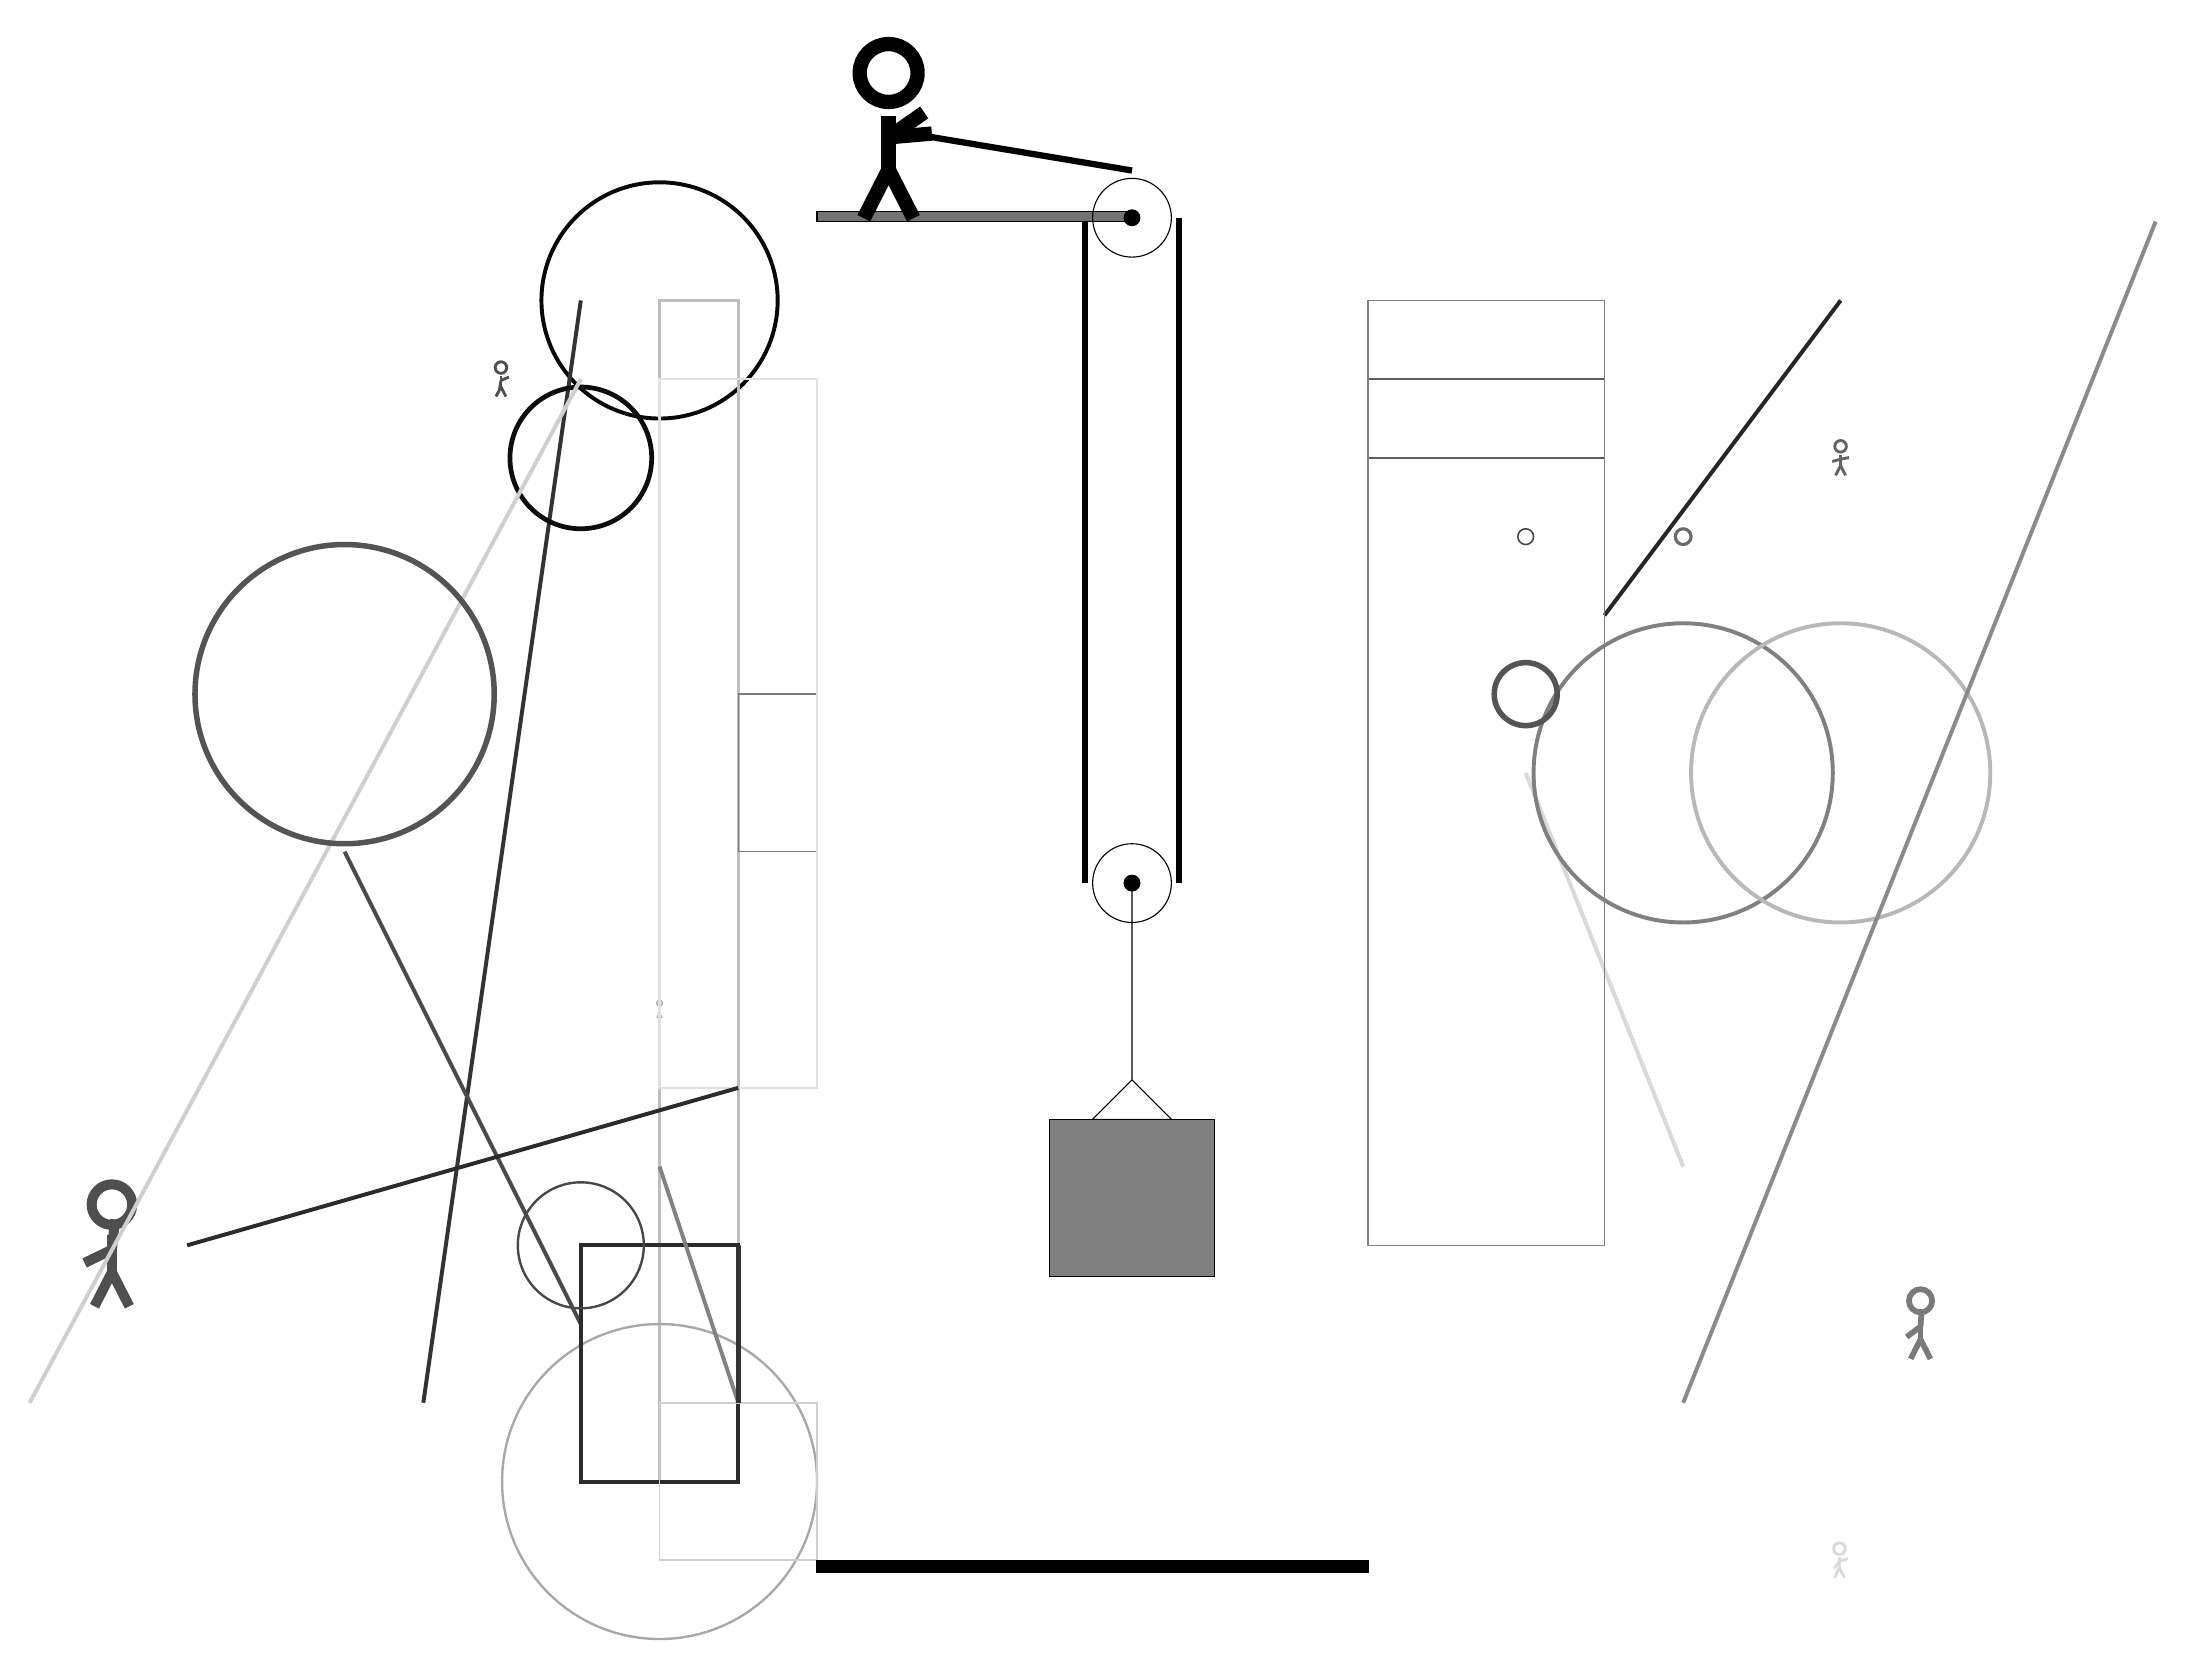
\begin{tikzpicture}
			%%%%% START %%%%%
			
			\draw[fill=black!55] (-2, 14) rectangle (2, 14.125);
			
			\draw (2, 5.6) circle (0.5);
			\draw[fill=black] (2, 5.6) circle (0.1);
			
			\draw (2, 14.05) circle (0.5);
			\draw[fill=black] (2, 14.05) circle (0.1);
			
			\draw [line width=0.5mm, color=black!97](-4, 13) circle (1.5);
			
			\draw[line width=0.4mm, color=black!26] (-3, 13) rectangle (-4, -2);
			\node[line width=0.5mm, color=black!33] at (-4, 4) {\Strichmaxerl[1][71][79]};
			\draw[line width=0.5mm, color=black!80](-5, 13) -- (-7, -1);
			\draw[line width=0.5mm, color=black!15](9, 2) -- (7, 7);
			\draw [line width=0.5mm, color=black!50](9, 7) circle (1.9);
			
			\draw[line width=0.2mm, color=black!52] (-3, 6) rectangle (-2, 8);
			
			\node[line width=0.2mm, color=black!61] at (11, 11) {\Strichmaxerl[2][16][11]};
			\draw [line width=0.6mm, color=black!95](-5, 11) circle (0.9);
			
			\node[line width=0.6mm, color=black!52] at (12, 0) {\Strichmaxerl[4][37][86]};
			\draw[line width=0.5mm, color=black!71](-5, 0) -- (-8, 6);
			\draw[line width=0.3mm, color=black!12] (-2, 12) rectangle (-4, 3);
			\draw[line width=0.2mm, color=black!63] (5, 12) rectangle (8, 11);
			
			\draw [line width=0.6mm, color=black!71](-11, 8) circle (0.0);
			\draw [line width=0.3mm, color=black!34](-4, -2) circle (2.0);
			\draw[line width=0.5mm, color=black!83] (-3, 1) rectangle (-5, -2);
			
			\draw [line width=0.2mm, color=black!73](7, 10) circle (0.1);
			\node[line width=0.2mm, color=black!15] at (11, -3) {\Strichmaxerl[2][54][19]};
			\draw [line width=0.7mm, color=black!67](7, 8) circle (0.4);
			\draw[line width=0.5mm, color=black!49](-4, 2) -- (-3, -1);
			\draw [line width=0.4mm, color=black!59](9, 10) circle (0.1);
			
			\draw [line width=0.5mm, color=black!28](11, 7) circle (1.9);
			
			\draw[line width=0.2mm, color=black!19] (-2, -3) rectangle (-4, -1);
			\draw[line width=0.7mm, color=black!80] (-3, 1) rectangle (-3, -1);
			\draw [line width=0.3mm, color=black!72](-5, 1) circle (0.8);
			
			\node[line width=0.2mm, color=black!69] at (-11, 1) {\Strichmaxerl[7][26][84]};
			
			\draw[line width=0.5mm, color=black!85](8, 9) -- (11, 13);
			\draw[line width=0.2mm, color=black!49] (5, 1) rectangle (8, 13);
			
			\draw[line width=0.5mm, color=black!46](9, -1) -- (15, 14);
			\draw[line width=0.5mm, color=black!19](-5, 12) -- (-12, -1);
			\draw [line width=0.7mm, color=black!67](-8, 8) circle (1.9);
			\draw[line width=0.5mm, color=black!83](-3, 3) -- (-10, 1);
			\node[line width=0.7mm, color=black!69] at (-6, 12) {\Strichmaxerl[2][81][23]};
			
			\draw (2, 5.6) -- (2, 3.1) -- (1.5, 2.6) -- (2.5, 2.6) -- (2, 3.1);
			\draw[fill=black!50] (0.95, 2.6) rectangle (3.05, 0.6);
			
			\draw[line width=0.8mm] (1.4, 14) -- (1.4, 5.6);
			\centerarc[line width=0.8mm](2, 5.6)(180:360:0.6);
			\draw[line width=0.8mm](2.6, 5.6) -- (2.6, 14.05);
			\centerarc[line width=0.8mm](2, 14.05)(0:90:0.6);
			\draw[line width=0.8mm](2, 14.65) -- (-1, 15.15);
			
			\node at (-1, 15.15) {\Strichmaxerl[10][-175][35]};
			
			\draw[fill=black] (-2, -3) rectangle (5, -3.15);
			
			%%%%% END %%%%%
		\end{tikzpicture}
	\end{figure}	
\end{document}